
\begin{figure}[ht]
\centering
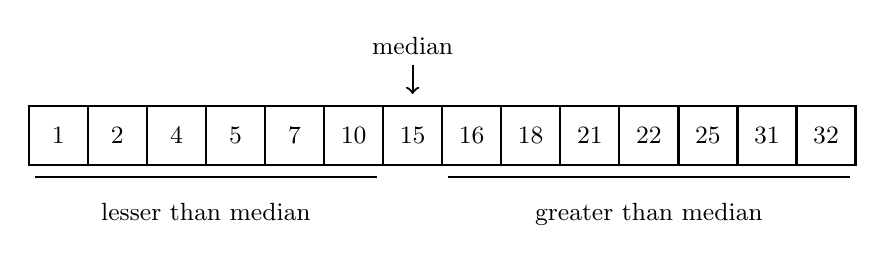
\begin{tikzpicture}[every node/.style={font=\small}, scale=0.75]

% --- Array values (10 elements) ---
\def\A{{1, 2, 4, 5, 7, 10, 15, 16, 18, 21, 22, 25, 31, 32}}
\def\MID{6} % Index of median (0-based): value = 23
% Draw array elements and indices
\foreach \i in {0,...,13} {
    \pgfmathsetmacro{\val}{\A[\i]}
    \draw[thick] (\i, 0) rectangle ++(1,1);
    \node at (\i+0.5, 0.5) {\val};
}

% Underline LEFT subarray (0..3)
\draw[thick] (0.1, -0.2) -- (6.0-0.1, -0.2);
% Label
\node[below=6pt] at (3, -0.2) {lesser than median};

% Underline RIGHT subarray (5..9)
\draw[thick] (7+0.1, -0.2) -- (13+1-0.1, -0.2);
% Label
\node[below=6pt] at (10.5, -0.2) {greater than median};

% Arrow for mid
\draw[<-, thick] (\MID+0.5, 1.2) -- +(0, 0.5) node[above] {median};

\end{tikzpicture}
\caption[Binary search]{Example of a sorted array containing 14 elements. }
\label{fig:binary-search-subarrays}
\end{figure}
